\documentclass[12pt,a4paper,twoside,titlepage]{article}
\usepackage[utf8]{inputenc}
\usepackage[english]{babel}
\usepackage{utopia}
\usepackage[margin=1in]{geometry}
\usepackage[parfill]{parskip}
\usepackage{makeidx}
\usepackage{graphicx}
\usepackage[onehalfspacing]{setspace}
\usepackage{fancyhdr}
%\usepackage{lastpage}
\usepackage{hyperref}
\renewcommand{\sffamily}{phv}

\newcommand{\titleText}{DHCP Aufgabe Dokumentation}
\newcommand{\authorText}{Patrick Günthard}
\newcommand{\dateText}{\today}

\title{\titleText}
\author{\authorText}
\date{\dateText}

\pagestyle{fancy}
\fancyhf{}

\fancyhead[EL]{\titleText}
\fancyhead[OR]{\authorText}
\cfoot{\thepage}% \space von \pageref{LastPage}}

\begin{document}
	\maketitle
	\tableofcontents

        \section{Software Basis}

        \begin{tabular}{|l|p{7cm}|}
          \hline
          \textbf{Server OS} & Debian GNU/Linux 8 Jessie (Im Text einfachheitshalber \textit{Debian-Server} oder \textit{Debian-System})\\\hline
          \textbf{Client OS} & Windows Server 2012 R2 (Im Text einfachheitshalber \textit{Windows-Client} oder \textit{Windows-System}) \\\hline
          \textbf{DHCP Server} & isc-dhcp-server \\\hline
        \end{tabular}

        \section{Aufgabenstellung}

        Die grundlegende Aufgabe bestand darin, auf einer Linux-VM einen DHCP Server zu installieren und diesen dann mit einem Windows-Client (ebenfalls auf einer VM) zu testen.

        \paragraph{Aufgaben}
        \begin{enumerate}
        \item Installation der VM
          \begin{itemize}
          \item Debian GNU/Linux 8
          \item Microsoft Windows Server 2012
          \end{itemize}
        \item Installation des DHCP Servers
        \item Konfiguration des Netzwerks
        \item Konfiguration des DHCP Servers
        \end{enumerate}

        \section{Vorgehen}

        \subsection{Hürden}

        Es gab verschiedene Hürden beim aufsetzten des DHCP-Servers. Zu begin war nicht klar, welches package installiert werden sollte, da im Debian-Repository mehrere Implementierungen vorhanden sind. Ich entschied mich dann für den \textit{isc-dhcp-server} welcher weit verbreitet ist.
        
        \subsection{Lösungen}
        
        \begin{figure}
        	\texttt{INTERFACES="eth1"}
        	\caption{\label{iscdhcpserver} Konfiguration der Datei auf dem Pfad \texttt{/etc/default/isc-dhcp-server}}
        \end{figure}
        
        \begin{figure}
        	\texttt{subnet 172.20.1.0 netmask 255.255.255.192 \{\\\space range 172.20.1.1 172.20.1.50;\\\}}\\
        	\caption{\label{dhcpdconf} Konfiguration des IP-Ranges in \texttt{/etc/dhcp/dhcpd.conf}}
        \end{figure}

        \begin{tabular}{lp{10cm}}
            DHCP Server & Das Packet \textit{isc-dhcp-server} eignet sich sehr gut für diese Aufgabe \\
            IP Konfiguration & Für eine korrekte verwendung muss die IP Adresse des Servers manuell gesetzt werden. Auf Unix-artigen Systemen wird dafür \textit{ifconfig} verwendet: \texttt{sudo ifconfig eth1 172.20.1.1 netmask 255.255.255.192}\\
            DHCP Konfiguration & Für die Konfiguration des DHCP Servers müssen 2 Dateien im \texttt{/etc/} modifiziert werden. Zum einen muss \texttt{/etc/default/isc-dhcp-server} modifiziert werden. Hier muss angegeben werden, auf welchem Netzwerk Interface der DHCP Server laufen wird. Wie schon im Beispiel der IP-Konfiguration wird hier das Interface \texttt{eth1} angegeben (Figure \ref{iscdhcpserver}). Auch muss die Datei \texttt{/etc/dhcp/dhcpd.conf} modifiziert werden (Figure \ref{dhcpdconf}). Hier muss die korrekte IP-Range definiert werden.
        \end{tabular}
        
        \section{Ergebnis \& Testprotokoll}

        \subsection{Ergebnis}

        \begin{figure}
          \center
          
          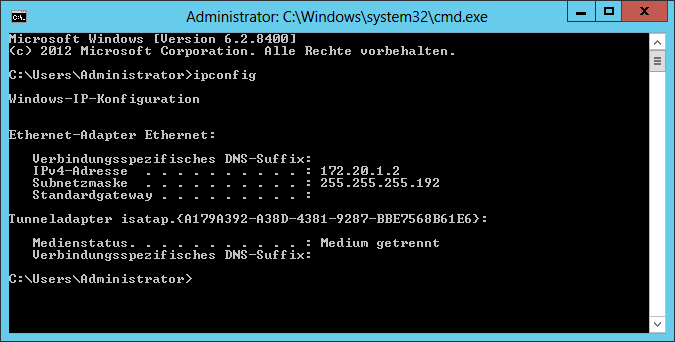
\includegraphics[width=8cm]{cmd_ipconfig_dynamic_ip}
          \caption{\label{dynip} Dynamisch zugewiesene IP auf Windows in \texttt{ipconfig}}
        \end{figure}

        \begin{figure}
          \center
          
          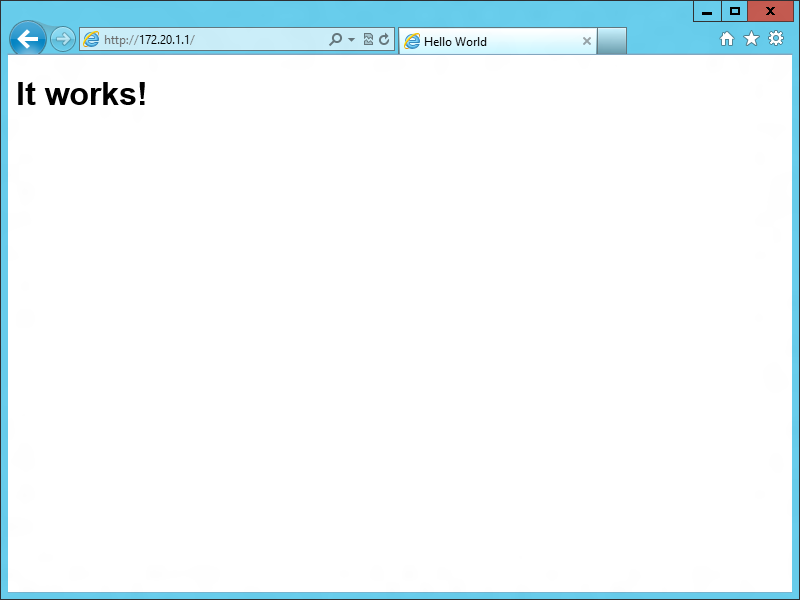
\includegraphics[width=8cm]{ie_web_example}
          \caption{\label{webserver} Erfolgreicher Zugriff vom Windows Client auf den Webserver auf dem Debian Server}
        \end{figure}
        
        Das Endergebnis war eine Debian 8 Maschine mit funktionierendem DHCP Server. Das richtige funktionieren des Servers wurde mit einem Windows-Client getestet welcher beim starten automatisch eine IP des im Server definierten Bereiches übernahm (Figure \ref{dynip}).

        Um zu testen ob auch eine Verbindung zwischen den beiden virtuellen Maschinen möglich ist, installierte ich auf dem Debian System ein Web-Server auf welchen ich auf dem Windows System erfolgreich zugreifen konnte (Figure \ref{webserver}).

        \subsection{Testprotokoll}


        \begin{tabular}{|l|l|p{5cm}|}
          \hline
          \textbf{Aufgabe} & \textbf{Status \ref{statusref}} & \textbf{Kommentar} \\\hline
          Server OS Aufsetzen & E & \begin{itemize}
          \item Debian
          \item Windows
          \end{itemize} \\\hline
        \end{tabular}

        \label{statusref}
        \textit{E} = erreicht, \textit{T} = teilweise erreicht, \textit{N} = nicht erreicht 
        
        \section{Reflexion}
        
        
\end{document}
